\documentclass{article}
\usepackage{url}
\usepackage{amsmath,bm}%
\usepackage{amsfonts}%
\pagestyle{empty}
\setlength{\textwidth}{7in}
\setlength{\oddsidemargin}{-.5in}
\setlength{\evensidemargin}{-.5in}
\setlength{\topmargin}{-.75in}
\setlength{\textheight}{9.25in}

\def\Var{\mathop{\rm Var\,}\nolimits}
\def\Cov{\mathop{\rm Cov\,}\nolimits}

\usepackage{Sweave}
\begin{document}

\begin{center}
{\bf STAT 515}

{\bf Homework \#5 WITH SOLUTIONS}

{\bf This homework must be submitted electronically to ANGEL.  I strongly
encourage the use of \LaTeX.}

\end{center}

\begin{enumerate}

\item Let $X_1$ and $X_2$ be independent exponential random variables with rates
$\lambda_1$ and $\lambda_2$, respectively. Let
\[
X_{(1)} = \min\{ X_1, X_2 \} \quad\mbox{and}\quad X_{(2)} = \max\{X_1, X_2 \}.
\]
We have shown in class that $X_{(1)}$ is exponential with rate
$\lambda_1+\lambda_2$.

  \begin{enumerate}
  
  \item Find $E X_{(2)}$. ({\bf Hint:} What is $E [ X_{(1)} + X_{(2)} ]$?)
  \begin{quotation}{\bf Solution:} Since $X_{(1)}+X_{(2)}=X_1 + X_2$, we conclude that
  \[
  E X_{(2)} = E(X_1+X_2)-E(X_{(1)}) = \frac{1}{\lambda_1} + \frac{1}{\lambda_2} - 
  \frac{1}{\lambda_1+\lambda_2}.
  \]
  \end{quotation}
  
  \item Find a probability density function for $X_{(2)}$ and use it to
  calculate $\Var X_{(2)}$.
  \begin{quotation}{\bf Solution:}
  Start with the cdf for $X_{(2)}$:
  \[
  F_{X_{(2)}}(x) = P(\max\{X_1, X_2\} \le x) = P(X_1\le x)P(X_2\le x) = (1-e^{-\lambda_1 x})
  (1-e^{-\lambda_2 x})
  \]
  Now differentiate to get a density function:
  \[
  f_{X_{(2)}}(x) = \frac{d}{dx} (1 - e^{-\lambda_1 x} - e^{-\lambda_2 x} + 
  e^{-(\lambda_1+\lambda_2) x}) = 
  \lambda_1 e^{-\lambda_1 x} +
  \lambda_2 e^{-\lambda_2 x} -
  (\lambda_1+\lambda_2) e^{-(\lambda_1+\lambda_2) x}.
  \]
  Interestingly, this is just the sum of two exponential densities minus a third!  We can use this fact to 
  find $E(X_{(2)}^2)$ quickly because we know that for an exponential random variable $Y$ with
  rate $\mu$, $E(Y^2)=\Var(Y) + [E(Y)]^2 = 2/\mu^2$:
  \[
  E(X_{(2)}^2) = \frac{2}{\lambda_1^2} + \frac{2}{\lambda_2^2} - \frac{2}{(\lambda_1+\lambda_2)^2}.
  \]
  We conclude that 
  \[
  \Var X_{(2)} = E(X_{(2)}^2) - [E X_{(2)}]^2 = 
  \frac{2}{\lambda_1^2} + \frac{2}{\lambda_2^2} - \frac{2}{(\lambda_1+\lambda_2)^2} -
  \left[\frac{1}{\lambda_1} + \frac{1}{\lambda_2} - \frac{1}{\lambda_1+\lambda_2}\right]^2.
  \]
  After simplification, we get
  \[
  \Var X_{(2)} = 
  \frac{1}{\lambda_1^2} + \frac{1}{\lambda_2^2} - \frac{3}{(\lambda_1+\lambda_2)^2}.
  \]
  \end{quotation}

  \item Find $\Cov (X_{(1)}, X_{(2)})$. ({\bf Hint:} What is $\Var[ X_{(1)} +
  X_{(2)} ]$?)
  \begin{quotation}{\bf Solution:}
  We know that $2\Cov(X_{(1)}, X_{(2)}) =  \Var[ X_{(1)} +  X_{(2)} ] - \Var X_{(1)}-
  \Var X_{(2)}$.
  Furthermore, $\Var [ X_{(1)} + X_{(2)} ]$ is simply $\Var X_1 + \Var X_2$ since $X_1$ and
  $X_2$ are independent and they have the same sum as $X_{(1)}$ and $X_{(2)}$.
  Thus,
  \[
  \Cov(X_{(1)}, X_{(2)}) = \frac12 \left( \frac{1}{\lambda_1^2} + \frac{1}{\lambda_2^2}
  - \frac{1}{(\lambda_1+\lambda_2)^2} - \Var X_{(2)}
  \right) = \frac{1}{(\lambda_1+\lambda_2)^2}.
  \]
  Actually, it is just as easy to find this covariance directly, since $E(X_{(1)}X_{(2)})=
  E(X_1X_2)=E(X_1)E(X_2)$:
  \[
  \Cov(X_{(1)}, X_{(2)}) = E(X_{(1)}X_{(2)}) - E(X_{(1)}) E (X_{(2)}) =
  \frac{1}{\lambda_1\lambda_2}
  - \frac{1}{\lambda_1+\lambda_2} \left( \frac{1}{\lambda_1} 
  + \frac{1}{\lambda_2} - \frac{1}{\lambda_1+\lambda_2} \right) =
  \frac{1}{(\lambda_1+\lambda_2)^2}.
  \]
  This also gives us a way to check that the answer for (b) is correct (!), since we could use
  this result as an alternative method of finding $\Var X_{(2)}$.
  \end{quotation}
  
  
  \end{enumerate}

\item Theorem~5.2 in Section~5.3.5 states that in a Poisson process $N(t)$ with
rate $\lambda$, given that $N(t)=n$, the n arrival times $S_1,\dots,S_n$ have
the same distribution as the order statistics corresponding to $n$ independent
random variables uniformly distributed on the interval $(0,t)$, i.e.,
$$P(S_1=t_1,\dots,S_n=t_n \mid N(t)=n)=\frac{n!}{t^n} I(0<t_1<\dots <t_n). $$

  \begin{enumerate}

  \item Clearly describe the general algorithm this suggests for simulating a
  Poisson process on an interval $[0,t]$. ({\bf Hint}: you will simulate the
  process in two stages.)
  \begin{quotation}{\bf Solution:}
  First, generate $N\sim\mbox{Poisson}(\lambda t)$, then generate $N$ i.i.d.~Uniform$(0, t)$
  variables, sort them, and take $S_1, \ldots, S_N$ to be the sorted values.
  \end{quotation}
  

  \item Consider a {\it homogeneous} Poisson process with $\lambda=10$. Using
  the algorithm from part (a), simulate 10,000 realizations of the above Poisson
  process on the interval $[0,5]$.
  \begin{quotation}{\bf Solution:}
  The trick here is storing a different number of arrival times for each realization.
  One way to do it using an R object called a list:
\begin{Schunk}
\begin{Sinput}
> X <- list()  # Use double-brackets to refer to list items, e.g., X[[1]]
> for (i in 1:10000) {
+   X[[i]] <- sort(runif(rpois(1, 50), min=0, max=5))
+ }
\end{Sinput}
\end{Schunk}
  \end{quotation}
  

  \item Report the sample mean for the number of events in the interval (0,1)
  and the number of events in the interval (4,5). How do these means compare
  with the corresponding theoretical expectations?
  \begin{quotation}{\bf Solution:}
  The R function {\tt sapply} is a helpful way to obtain these answers.  Since these are sample
  means, I'll report them as 95\% confidence intervals:
\begin{Schunk}
\begin{Sinput}
> f0 <- function(vec) sum(0<vec & 1>vec)
> ans0 <- sapply(X, f0)
> mean(ans0) + c(-1, 1) * 1.96 * sd(ans0)/ sqrt(length(ans0))
\end{Sinput}
\begin{Soutput}
[1]  9.891992 10.015608
\end{Soutput}
\begin{Sinput}
> f4 <- function(vec) sum(4<vec & 5>vec)
> ans4 <- sapply(X, f4)
> mean(ans4) + c(-1, 1) * 1.96 * sd(ans4)/ sqrt(length(ans4))
\end{Sinput}
\begin{Soutput}
[1]  9.936118 10.059882
\end{Soutput}
\end{Schunk}
  \end{quotation}
  

  \item Plot a histogram each for the distribution of the number of events in
  the interval (0,1) and the interval (4,5) respectively, based on the 10,000
  realizations.
  \begin{quotation}{\bf Solution:}
  Although it was not required, the code below produces histograms with 
  the true theoretical Poisson counts superimposed:
\begin{Schunk}
\begin{Sinput}
> par(mfrow=c(1,2))
> hist(ans0, breaks=0.5+(min(ans0)-1):max(ans0))
> x0 <- min(ans0):max(ans0)
> lines(x0, 10000*dpois(x0, 10), col=2, type="b")
> hist(ans4, breaks=0.5+(min(ans4)-1):max(ans4))
> x4 <- min(ans4):max(ans4)
> lines(x4, 10000*dpois(x4, 10), col=2, type="b")
\end{Sinput}
\end{Schunk}
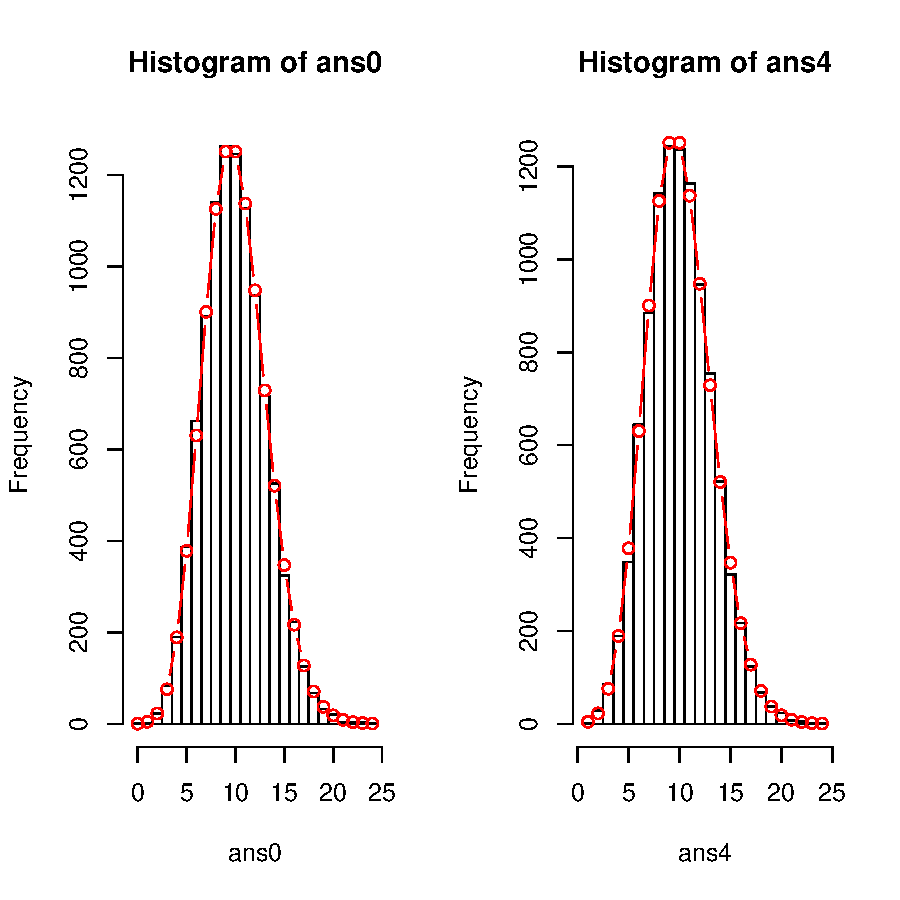
\includegraphics{sol05-003}
  \end{quotation}
  

  \end{enumerate}

\item Cars pass a certain street location according to a Poisson process with
rate $\lambda$. A woman who wants to cross the street at that location waits
until she can see that no cars will come by in the next $T$ time units.

  \begin{enumerate}

  \item Find the probability that her waiting time is 0.
  \begin{quotation}{\bf Solution:}
  This is the probability that the first car will take longer than $T$ to arrive, which
  is $e^{-\lambda T}$.
  \end{quotation}
  

  \item Find her expected waiting time.
  \begin{quotation}{\bf Solution:}
  Let $N$ be the number of cars that pass before she can cross.  Since each passing car 
  restarts the waiting, part (a) tells us that $N$ is the same as the number
  of independent Bernoulli$(e^{-\lambda T})$ trials before the first success occurs.  
  We conclude that $N+1$ has a geometric distribution with mean $e^{\lambda T}$,
  so $E(N)=e^{\lambda T}-1$.

  Now, for a car that passes in less than $T$ time units,
  if $X$ is the total waiting time, then $E X = E[E(X\mid N)]$.  We know
  that $E(X \mid N)$ is simply $N$ times the expectation of a single passing
  time, given that the time is less than $T$.  To find the latter, we may integrate the
  conditional density of an exponential, say $Y$, given that $Y\le T$:
  \[
  E(Y \mid Y \le T) = \frac{1}{1-e^{-\lambda T}} \int_0 ^T y \lambda e^{-\lambda y} \,dy
  = \frac{1-e^{-\lambda T}(\lambda T+1)}{\lambda(1-e^{-\lambda T})}
  \]
  We conclude that $E(X)$ is $E(N)$ times the above expression:
  \[
  E(X) = \frac{(e^{\lambda T}-1)[1-e^{-\lambda T}(\lambda T+1)]}
  {\lambda(1-e^{-\lambda T})} =
  \frac{e^{\lambda T} - \lambda T - 1}{\lambda}.
  \]
  \end{quotation}
  

  \end{enumerate}

\end{enumerate}

\end{document}

